\documentclass{article}

% Language setting. Replace `english' with e.g. `spanish' to typeset the
% document in another language: it decides hyphenation and the words LaTeX
% writes itself, such as "Figure" and "Contents".
\usepackage[english]{babel}

% Page size and margins. Replace `letterpaper' with `a4paper' outside the US.
\usepackage[letterpaper,top=2cm,bottom=2cm,left=3cm,right=3cm,marginparwidth=1.75cm]{geometry}

% The packages this example uses.
\usepackage{amsmath}    % maths
\usepackage{graphicx}   % images
\usepackage[colorlinks=true, allcolors=blue]{hyperref}

\title{Your Paper}
\author{You}

\begin{document}
\maketitle

\begin{abstract}
This is an example project. Every part of it is a thing you are likely to
want, shown once: sections, an image, a table, some mathematics, and a
citation. Delete what you do not need --- or delete all of it and start from
an empty page.
\end{abstract}

\section{Introduction}

The file you are reading is \verb|main.tex|, and it is the one that gets
compiled. The other files in this project are the ones it refers to: an image
and a list of references. You can add more from the file tree on the left, or
by dragging them onto it.

Press \textbf{Recompile} to build the document. The PDF appears on the right,
and double-clicking a paragraph in it will put the cursor on the line that
produced it. Anything LaTeX complains about is listed under the PDF.

\section{Sections and subsections}
\label{sec:sections}

Use \verb|\section| and \verb|\subsection|, as this document does. The
numbering and the table of contents are worked out for you, so moving a
section moves everything that refers to it.

\subsection{Referring to things}

Give something a label and refer to it by that label rather than by its
number: see Section~\ref{sec:sections}, Figure~\ref{fig:frog} and
Table~\ref{tab:widgets}. The numbers are then never wrong, however much the
document is rearranged.

\section{Images}

Figure~\ref{fig:frog} is \verb|frog.jpg|, which is in this project. Upload
your own images from the file tree and refer to them the same way.

\begin{figure}[h]
\centering
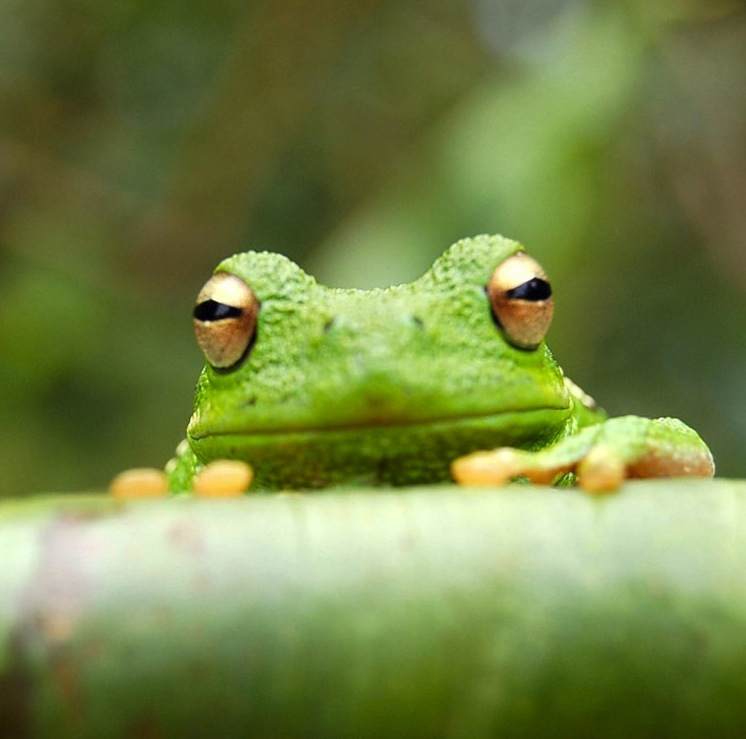
\includegraphics[width=0.3\textwidth]{frog.jpg}
\caption{\label{fig:frog}A frog photographed by an unknown photographer.}
\end{figure}

The \verb|[h]| asks for the figure to go here; LaTeX will move it if the page
would look wrong, which is usually the right decision. The width is given as a
fraction of the text width so that it stays right if the margins change.

\section{Tables}

\begin{table}[h]
\centering
\begin{tabular}{lrr}
\hline
Item      & Quantity & Unit price \\
\hline
Widget    & 3        & 7.50 \\
Gadget    & 12       & 1.25 \\
Doohickey & 1        & 42.00 \\
\hline
\end{tabular}
\caption{\label{tab:widgets}An example table.}
\end{table}

The column specification \verb|{lrr}| is one letter per column: \verb|l| for
left-aligned, \verb|r| for right-aligned, \verb|c| for centred. Numbers read
better right-aligned, which is why the last two columns are.

\section{Mathematics}

Maths goes between dollar signs when it belongs in a sentence, like
$E = mc^2$, and in an environment when it deserves a line of its own:

\begin{equation}
\label{eq:gaussian}
\int_{-\infty}^{\infty} e^{-x^2} \, dx = \sqrt{\pi}.
\end{equation}

Equation~\ref{eq:gaussian} is numbered because it is in an \verb|equation|
environment. Use \verb|equation*| for one that is not.

\section{Citations}

Put your references in a \verb|.bib| file --- this project has
\verb|sample.bib| --- and cite them by key, like this: \cite{greenwade93}.
Lamport's book \cite{lamport94} is the one to read next.

The bibliography at the end is generated from the entries you actually cite,
in the style named by \verb|\bibliographystyle|.

\section{Getting help}

Anything you cannot remember the syntax for is probably a button on the
toolbar above the text. The rest is in the LaTeX documentation, and it is
worth reading the part about whatever you are doing before you fight it.

\bibliographystyle{alpha}
\bibliography{sample}

\end{document}
